\documentclass[a4paper, 12pt]{article}

\usepackage{fontspec}   %加這個就可以設定字體
\usepackage{xeCJK}      %讓中英文字體分開設置
\usepackage{zhnumber}
\usepackage{indentfirst}
\usepackage{listings}
\usepackage{float}
\usepackage{graphicx}
\usepackage{caption}
\usepackage{fancyhdr}
\usepackage{hyperref}
\usepackage{amsmath}
\usepackage{multirow}
\usepackage[dvipsnames]{xcolor}
\usepackage{graphicx}
\usepackage{subcaption}
\usepackage{etoolbox}
\usepackage{tcolorbox}
\usepackage{multicol}
\usepackage{tabularx}
\usepackage[toc]{appendix}
\usepackage{titlesec}
\usepackage{titling}
\usepackage{newunicodechar}
\usepackage{hhline}
\usepackage{tocloft} % adding the tocloft package for toc customization

\usepackage[english]{babel}
\usepackage[autostyle]{csquotes}

\usepackage[sorting=nty]{biblatex}


\renewcommand\appendixtocname{附錄}


\addbibresource{ref.bib}

\setcounter{tocdepth}{5}
\setcounter{secnumdepth}{5}

\renewcommand\tabularxcolumn[1]{m{#1}}% for vertical centering text in X column
\newcolumntype{Y}{>{\centering\arraybackslash}X}


\usepackage[
  top=2cm,
  bottom=2cm,
  left=2cm,
  right=2cm,
%  headheight=17pt, % as per the warning by fancyhdr
%  includehead,
  includefoot,
  heightrounded, % to avoid spurious underfull messages
]{geometry} 

\newcounter{mysec}[section]
\renewcommand\thesection{%
    \addtocounter{mysec}{1}%
    \zhnum[style={Traditional,Financial}]{mysec}、}
\renewcommand\thesubsection{\zhnum{subsection}、} % added a 、
\renewcommand\thesubsubsection{(\zhnum{subsubsection})} % added parentheses
% (full-width, don't know if that's what you want)
\renewcommand\theparagraph{} % you don't want paragraph numbers
\renewcommand\thesubparagraph{} % nor subparagraph numbers

% we have to adjust the spacing in the toc because the section label is longer than usual
\addtolength\cftsecnumwidth{1em}
\addtolength\cftsubsecindent{1em}
\addtolength\cftsubsubsecindent{1em}

% here we need to make sure the normal section counter is accessed
\titleformat{\section}{\Large\bfseries\filcenter}
    {\zhnum[style={Traditional,Financial}]{section}、}{.5em}{}
% not really sure what you intend to achieve with \fontsize but I'll leave it here
\titleformat*{\subsection}{\fontsize{12}{12}\bfseries} 
\titleformat*{\subsubsection}{\fontsize{12}{12}\bfseries}

% no extra version for numberless is necessary since no numbers are used anyways
% also you get newlines from omitting the [display] in \titleformat already
\titleformat{\paragraph}
    {\fontsize{14}{14}\bfseries}{}{0em}{} 
\titleformat{\subparagraph}
    {\fontsize{12}{12}\bfseries}{}{0em}{}
% we need the following so that they don't indent (second argument, 0em);
% you'll have to adjust the spacing though since this is not display style anymore:
\titlespacing*{\paragraph}{0em}{3.25ex plus 1ex minus .2ex}{.75ex plus .1ex} 
\titlespacing*{\subparagraph}{0em}{3.25ex plus 1ex minus .2ex}{.75ex plus .1ex}

\renewcommand{\maketitlehooka}{\sffamily}

\renewcommand{\baselinestretch}{1.5}

\pagestyle{fancy}
\renewcommand{\headrulewidth}{0pt}
\fancyfoot{}
\fancyhead{}
\cfoot{\footnotesize \thepage}

\addto\captionsenglish{%
  \renewcommand\appendixname{附錄}
  \renewcommand\appendixpagename{附錄}
  \renewcommand{\contentsname}{目錄}
  \renewcommand{\figurename}{圖}
}

\captionsetup[table]{name=表}
%\lhead{利用VAE-pix2pix生成擬真的山脈模型}
%\rhead{2021臺灣國際科學展覽會研究報告}


\lstset{basicstyle=\ttfamily, keywordstyle=\bfseries}

\setCJKmainfont{Noto Serif CJK TC}
\setmainfont{Times New Roman}
\setmonofont{Consolas}
% \setmonofont{Cascadia Code}
\XeTeXlinebreaklocale "zh"             %這兩行一定要加,中文才能自動換行
\XeTeXlinebreakskip = 0pt plus 1pt     %這兩行一定要加,中文才能自動換行
\title{利用VAE-pix2pix生成擬真的山脈模型}
\author{程品奕、李杰穎}
% \date{中華民國} %不要日期

\setlength{\parindent}{2em}
\setlength{\parskip}{0.5em}


\renewcommand{\thefootnote}{\roman{footnote}}

\begin{document}

\pagenumbering{roman}

\tableofcontents
\newpage

\begin{abstract}

In this study, we use NASA’s SRTM 1 Arc-Second dataset to collect altitude maps from around the world, and we also use MapTiler to collect corresponding satellite images. Using these collected images, we trained our VAE-pix2pix model, which is a Variational Autoencoder (VAE) combined with pix2pix (a Conditional Generative Adversarial Network). VAE-pix2pix can add details of the real-world mountain should have (including sharp ridges, mountain wall textures, continuous river networks, etc.) to the heightmap, users draw which. Our model can generate the corresponding satellite images as well. Compared with the original pix2pix model, our model can generate heightmap and satellite images that are more realistic. It can also generate different styles of heightmap and satellite images by changing the value of the latent code, such as the color of the landform or the height of the snow line, and even can generate styles that are probably do not exist in the real world. All this work increases the diversity of the images generated by the model. To make our model can be better used, we have developed a client on Unity, which can generate a mesh that allows users to directly use it when developing the game in Unity. In conclusion, our work has simplified generating a realistic mountain model in the game or other fields as well.

\end{abstract}

\renewcommand{\abstractname}{摘要}
\begin{abstract}

本研究利用NASA的SRTM 1 Arc-Second資料集來收集全球各地的地形高度圖(heightmap),也利用MapTiler網站收集相對應的衛星空照圖,用這些收集的圖像,訓練我們建構的VAE-pix2pix模型。VAE-pix2pix為Variational Autoencoder (VAE)及pix2pix (為一個Conditional Generative Adversarial Network)結合的模型,能將人工繪製的高度圖加上真實山脈應有的細節(包含尖銳的山脊、山壁上的紋路、連續的河流網路等……),並生成出相對應的擬真衛星空照圖。相較於原pix2pix模型,VAE-pix2pix所生成的高度圖及衛星空照圖會更接近於真實世界的地形高度圖及衛星空照圖,同時VAE-pix2pix模型也能透過改變latent code的數值來生成出不同風格的高度圖及空照圖,如地貌的顏色或雪線的高度等,甚至能生成出可能不真實存在的地形風格,這些都增加模型生成圖像的多樣性。為了使我們建構的模型能更廣泛的被應用,我們在Unity上開發了Unity客戶端,其生成的mesh可以讓使用者直接應用於遊戲的場景,簡化了遊戲中生成擬真山脈模型的任務。

\end{abstract}

\newpage
\pagenumbering{arabic}

\section{前言}
\subsection{研究動機}
隨著3C的普及,遊戲已經成為現代人打發時間、舒壓及社交的必需品;隨著科技技術的進步,對於遊戲畫質的要求也越高,而在製作各種遊戲時,常常會需要生成擬真的地形作為遊戲的場景。

傳統上,遊戲的擬真山脈地形是透過人工繪製。在將大致的架構畫出來後,還需花費不少時間捏出山脊和挖出河流等細節部分。而近年來,人工智慧演算法在圖像的生成上有重大的突破,不論是生成圖片或是將影像的風格提取出來,並轉換到另一張影像,都已經是可行的方法,因此本研究希望簡化人工繪製的過程,透過訓練生成對抗網路來達到生成擬真山脈地形的成果。

\subsection{研究目的}
本研究期望能簡化遊戲製作者在生成擬真山脈地形模型的流程,同時確保生成擬真山脈的效果。在製作3D地形模型時,需要\textbf{高度圖 (heightmap)}來指定地表的形狀,以及\textbf{紋理貼圖(texture)} 來指定地表的顏色,傳統的方法是需要設計師一筆一畫來畫出山脈的細節及風格。本研究期望能建構出一個類神經網路模型,自動畫出山脈的細節及風格。在輸入圖像部分,使用者不需繪製山脈的細節及風格,只需要繪製一張人工手繪的\textbf{大致地形架構}並提供一組\textbf{風格參數},將其輸入訓練好的VAE-pix2pix模型,即可生成出細節豐富的地形高度圖和紋理貼圖,供建立3D地形模型時使用。
\section{研究過程與方法}
\subsection{文獻探討}
\subsubsection{物理侵蝕模型}
一般來說,若要提升遊戲中山脈地形的真實度,其中一種方法為使用侵蝕的物理模型,如論文\cite{jako2011fast},建構一個物理模型,模擬水流在地形上侵蝕與堆積,論文作者藉由此模型結合GPU,實現改變地形樣貌的效果。

根據論文\cite{jako2011fast}的內所敘述的物理模型,本研究利用PyTorch實現論文\cite{jako2011fast}所述之物理侵蝕模型,之後會將其與經訓練的VAE-pix2pix模型進行真實度及實用性的比較。

此物理侵蝕模型將地表分成正方形的網格,使用歐拉法求地表上每格的水深、含沙量和網格間的水流速,並根據水量和流速進行侵蝕和堆積,疊代多次後可得出侵蝕一段時間後的地面和水面高度圖。一次疊代的步驟如下:

\begin{enumerate}
    \item 在每個網格加上等量的水,模擬均勻的降雨
    \item 更新流速(加速度受坡度和阻力影響)
    \item 根據流速讓水流到鄰近的格子,同時搬運等比例的砂土
    \item 根據水量和流速進行侵蝕,增加水中含沙量,降低地面高度
    \item 將水中一定比例的沙土堆積到地面
    \item 移除每格一定比例的水,模擬蒸發
\end{enumerate}


\begin{figure}[H]
    \centering
    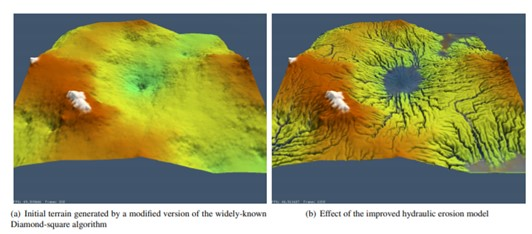
\includegraphics[width=\linewidth]{fig/1.jpg}
    \caption{物理侵蝕模型的效果 (取自\cite{jako2011fast})}
    \label{fig:1}
\end{figure}


\subsubsection{pix2pix模型}
論文\cite{isola2017image}則為pix2pix,是一個Conditional generative adversarial network(又稱 Conditional GAN)。pix2pix 的用途是把圖像轉換成一種特定的風格,或是依據邊緣或色塊等標籤生成擬真圖像。

pix2pix訓練時需要成對的影像資料,而模型的目標則是將第一張圖片轉換為第二張圖片。例如圖二,即為pix2pix可做到的各種應用,而pix2pix模型的目標是將左圖做為輸入,輸出右邊的圖像。

\begin{figure}[H]
    \centering
    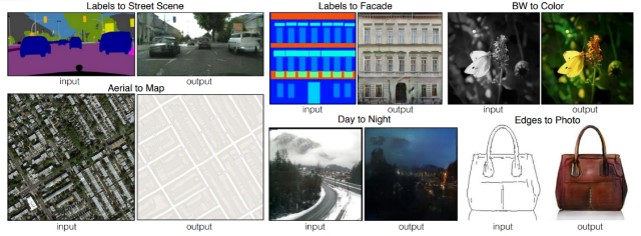
\includegraphics[width=\linewidth]{fig/2.jpg}
    \caption{pix2pix可做到的圖像風格轉換(取自\cite{isola2017image})}
    \label{fig:2}
\end{figure}

pix2pix模型由generator和discriminator兩個部分組成。generator 的結構為U-Net,訓練時會嘗試把輸入圖像轉換為目標圖像。discriminator則是一個分類器,訓練時會嘗試分辨哪些圖是generator生成的圖,哪些是真的目標圖像。兩者會同時訓練,generator生成的圖越不容易被discriminator分辨出來,就代表generator表現得越好。利用這點來訓練generator,就能讓它的輸出盡可能的真實。

\begin{figure}[H]
    \centering
    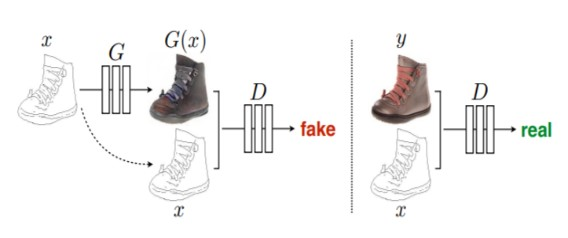
\includegraphics[width=0.6\linewidth]{fig/3.jpg}
    \caption{訓練Conditional GAN將鞋子的邊緣圖生成實際鞋子的圖像。(取自\cite{isola2017image})}
    \label{fig:3}
\end{figure}

如圖三中,discriminator的任務是辨認出哪些圖片是由generator所生成(如左),哪些是原始圖像(如右)。我們的研究將使用pix2pix作為基礎模型。

\subsubsection{VAE (Variational Autoencoder)}
Autoencoder模型為Encoder-decoder結構。運作時,輸入圖片x會被encoder編碼成latent code,再由decoder依照latent code的資訊嘗試還原出x。Latent code為整個模型結構的瓶頸,所以encoder的目標是把輸入x以最少資訊損失的方式壓縮成維數相對很小的latent code,以供decoder使用。也就是說,encoder做的是非線性降維,它會萃取輸入圖片的高階特徵。


\begin{figure}[H]
    \centering
    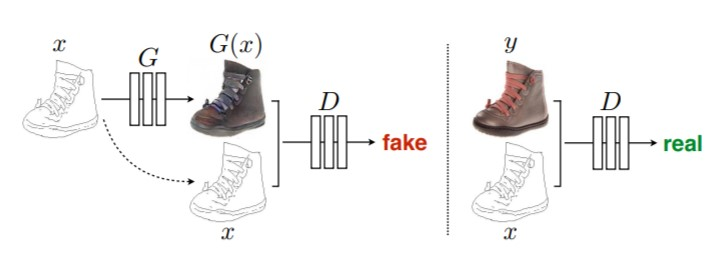
\includegraphics[width=0.5\linewidth]{fig/4.jpg}
    \caption{VAE的基本模型結構}
    \label{fig:4}
\end{figure}

而VAE(Variational Autoencoder)[7]類似Autoencoder,但其中encoder的輸出為平均及標準差,這兩個參數代表著一個高斯分布,訓練時latent code會從該分布中隨機取出,傳給decoder。且latent code的先驗分布會被額外的latent loss拉成接近標準高斯分布的形狀,這項限制使VAE能學到更有意義的latent space,也方便應用。其基本模型結構如圖六。

生成擬真的人臉圖像即為VAE典型的應用,而VAE學習到的latent space中,各維度的意義可能是臉的方向、膚色、頭髮長度或眼睛大小。
我們的研究將以VAE與pix2pix結合,成為一種新的類神經網路架構,接著會以這個架構訓練能生成地形高度圖和紋理貼圖的模型,最後會與基礎的pix2pix模型與物理侵蝕模型進行生成品質的比較。

\subsection{收集訓練模型所需之圖像資料}
本研究主要會收集五個地區的地形高度圖及空照圖。這個五個地區分別為橫斷山脈、喜馬拉雅山、祕魯安地斯山脈、阿根廷及加拿大的冰河地形。透過收集不同區域的地形,使VAE-pix2pix能學到不同地區的高度圖及空照圖的特徵。
\subsubsection{地形高度圖}
地形高度圖的資料來源為NASA的SRTM 1 Arc-Second資料集\cite{srtm1arc}。此資料集將1經度 $\times$ 1緯度範圍的高度資料儲存為一張高度圖,每張高度圖的編號方式是按照其高度圖左下角的座標作為檔名,若此張高度圖的收集範圍為25°N, 98°E、25°N, 99°E、24°N, 99°E、24°N, 98°E四個座標點所圍成的範圍,則此張高度圖的檔名即為N24E98,我們在附錄中會使用這種方式來表示各地區的收集範圍。

因為SRTM資料集採用特殊的HGT格式,不能使用一般的圖像軟體讀取,也就無法作為模型的訓練資料,所以我們利用gmalthgtparser來將HGT格式轉為可以直接以圖像軟體讀取的PNG格式。gmalthgtparser為一個Python module,可以讀取HGT檔案中特定地點的高度值(單位為公尺),讀取到高度值後,我們利用式~\ref{eq:1}~將高度值轉為RGB值。

\begin{equation}
    (R, G, B)=\left(\left\lfloor\frac{\text {height}}{256^{2}}\right\rfloor,\left\lfloor\frac{\text {height } \% 256^{2}}{256^{1}}\right\rfloor,\left\lfloor\frac{\text {height } \% 256}{1}\right\rfloor\right)
    \label{eq:1}
\end{equation}

式~\ref{eq:1}~中的$\text{height}$代表真實高度值,而$R,G,B$分別對應到圖檔的三個顏色通道。

對高度值進行轉換後,我們即可以將一張HGT檔案的高度圖轉換為方便易用的PNG高度圖,轉換後的PNG高度圖如圖~\ref{fig:5}~。

\begin{figure}[H]
    \centering
    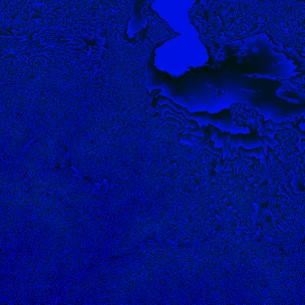
\includegraphics[width=0.45\linewidth]{fig/5.jpg}
    \caption{由HGT檔案轉換的PNG高度圖}
    \label{fig:5}
\end{figure}

\subsubsection{衛星空照圖}
本研究中,地形高度圖需要與衛星空照圖相互對應,所以使用MapTiler所提供的XYZ tiles map來收集衛星空照圖。XYZ tiles map是一種儲存地圖資料的方式,其方式為將大圖切割成許多張小圖,可以使地圖加載的速度變快,亦可節省網路資源。我們利用MapTiler所提供的衛星空照圖tiles map服務,收集橫斷山脈範圍內的多張衛星空照圖,再以EPSG:4326 (WGS 84)座標系統將各張小圖(tiles)組合成一張與地形高度圖互相對應的衛星空照圖。

因為衛星空照圖需與地形高度圖相互對應,所以空照圖的收集數量要與高度圖相同。表一為收集五個地區的高度圖及空照圖數量,具體的收集範圍列於附錄A:

\begin{table}[H]
    \centering
    \caption{五個地區的高度圖及空照圖收集總數 (單位:張)}
    \begin{tabularx}{\linewidth}{|Y|Y|Y|}
        \hline
        地區           & 高度圖數量 & 空照圖數量 \\ \hhline{|=|=|=|}
        橫斷山脈       & 16         & 16         \\ \hline
        喜馬拉雅山     & 10         & 10         \\ \hline
        祕魯安地斯山   & 15         & 15         \\ \hline
        阿根廷冰河地形 & 9          & 9          \\ \hline
        加拿大冰河地形 & 5          & 5          \\ \hline
    \end{tabularx}
    \label{tab:2}
\end{table}

\subsection{本研究建構的模型結構 — VAE-pix2pix}
本研究的目的是簡化人工繪製地形的過程。我們建構一個類神經網路模型,以人工繪製的大致地形架構作為輸入,生成擬真的高度圖和紋理貼圖供遊戲開發者使用。

我們將蒐集到的真實高度圖用中值模糊處理,把山脊上的小河谷和大河谷上的小凸起物抹除,以模擬手繪大致山脈的架構。訓練時,這張\textbf{模糊高度圖}就做為pix2pix模型的輸入,未經模糊處理的\textbf{真實高度圖}和與之對應的\textbf{衛星空照圖}則做為pix2pix模型的目標輸出。

但如果僅使用原pix2pix模型來訓練,因為pix2pix本身缺乏調整生成風格的機制,所以應用時將無法任意的調整生成地形的風格,限制了應用彈性。為了讓模型能調整生成風格,我們建構了\textbf{VAE-pix2pix模型},在pix2pix的U-Net前增加了style encoder (為VAE的encoder)。訓練時,style encoder負責從高度圖和空照圖提取出這些風格資訊(latent code)輸入U-Net,再由U-Net以正確的風格生成高度圖和空照圖。latent code也會提供給discriminator(此路徑不接收反向傳播的梯度),以利判斷U-Net是否生成正確的風格。而應用時,使用者只要輸入給U-Net不同風格資訊,就能控制它生成不同風格的地形。

從VAE的角度來看,此模型相當於利用U-Net作為Decoder,並在瓶頸處額外輸入高度圖作為空間資訊的VAE。

\begin{figure}[H]
    \centering
    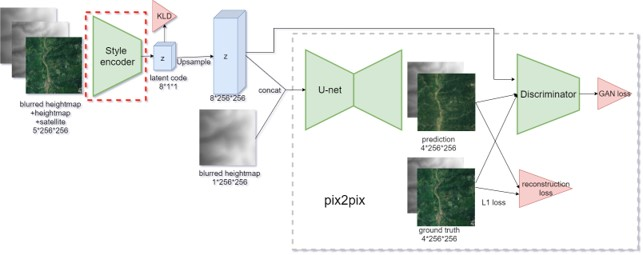
\includegraphics[width=\linewidth]{fig/6.jpg}
    \caption{pix2pix和VAE-pix2pix的訓練及應用流程簡圖}
    \label{fig:6}
\end{figure}

\begin{figure}[H]
    \centering
    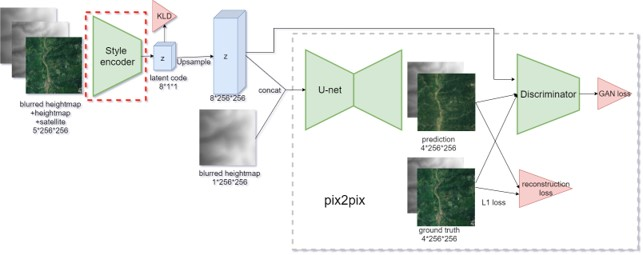
\includegraphics[width=\linewidth]{fig/7.jpg}
    \caption{VAE-pix2pix整體模型結構}
    \label{fig:7}
\end{figure}


為了不限制能處理的圖片大小,並允許使用者在不同位置指定不同風格,本研究的style encoder不會像典型的VAE一樣使用fully connected layer來產生latent code,而是用convolution layer,以保留空間維度。

因為style encoder的輸入中含有目標空照圖(ground truth) 的資訊,所以作為瓶頸的latent code必須足夠窄,以防止U-Net輕易的將目標高度圖和空照圖直接輸出。如果輸入圖的長寬為h, w,則style encoder會將latent code縮小到一個有8 channels,長為 (h/256),寬為(w/256)的tensor。

設計模型結構時,一開始的style encoder是無跳躍連結(skip-connections)的多層CNN,但我們發現如果不在style encoder中使用batch normalization (BN),訓練過程中會造成梯度爆炸;但如果使用BN,則會造成latent code梯度消失和KLD vanishing,也就是style encoder退化成只會輸出標準高斯分布的latent code。我們認為這個現象很有可能是因為style encoder中,接近後端的BN使產生的latent code過於不穩定,導致U-Net不採納latent code,只參考模糊高度圖。為了解決這個問題,我們用類似ResNet的方式,把每一組[conv, ReLU, bn] block的旁邊加上一條路徑,使資料可以選擇路徑,不一定要經過導致不穩定的BN,同時,因為這條路徑上沒有可訓練的bias或weight,所以不會像直接去除BN的時候一樣發生梯度爆炸。

\begin{figure}[H]
    \centering
    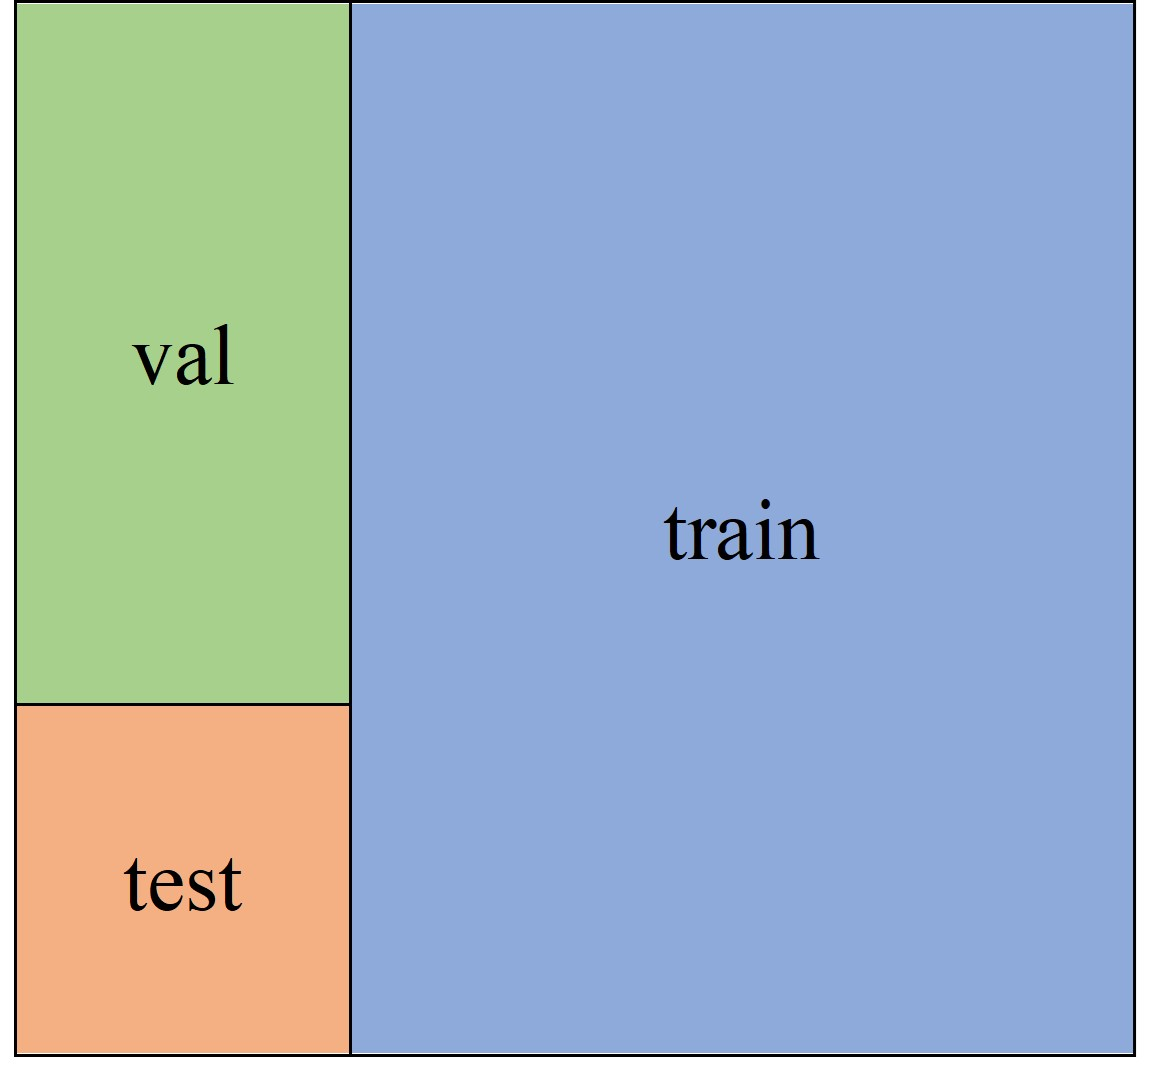
\includegraphics[width=0.4\linewidth]{fig/8.jpg}
    \caption{Style encoder的具體結構}
    \label{fig:7}
\end{figure}

\subsection{對U-Net的修改}
為了讓VAE-pix2pix模型能更符合我們的需求,我們對U-Net進行修改,修改的項目如下:

\subsubsection{Convolution Layer 的 stride}
原本pix2pix的每個convolution layer的stride都是設為2,這樣會使feature map每往下一層都縮小成0.5倍,以處裡更大範圍的特徵。但是在生成地形這項工作中,只需要產生較小範圍的細節,且全局特徵已經能從模糊高度圖和style encoder得到,所以我們把U-Net改成每兩層convolution layer才會有一個是stride為2 (另一個是stride為1),使U-Net更專注於精細特徵。不過此設定增加了feature map大小,使訓練時間變成原本的約4倍。

\subsubsection{激勵函數tanh}

U-Net會輸出一張高度圖和一張紋理貼圖,其中高度圖的像素值不應被U-Net尾端的tanh運算限制,所以我們把tanh改成只會對空照圖運算。

\subsection{生成訓練資料集}

我們將收集的高度圖和空照圖分為train、test兩個區域 (train用於訓練模型,而test則用來在訓練完成後用於測試模型),並分別從這兩個區域中切割出訓練資料集的圖像。這樣可以使個兩個部分的圖像不重複,以測試模型的精準度。

\begin{figure}[H]
    \centering
    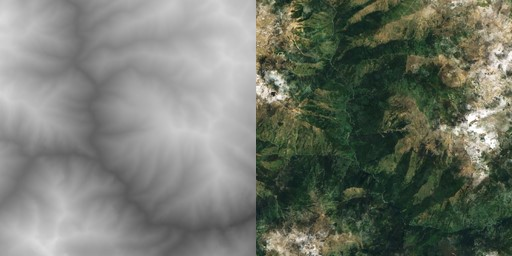
\includegraphics[width=0.3\linewidth]{fig/9.jpg}
    \caption{train、test在大圖的位置}
    \label{fig:9}
\end{figure}

將收集的空照圖及高度圖分隔成上述兩個區域後,我們隨機在其上切割出多個大小為256 x 256像素的高度圖及空照圖。並將高度圖透過線性變換的方式由24 bits高度圖轉換為8 bits的高度圖。後再利用中值模糊 (median blur)將真實高度圖模糊為模糊高度圖,以模擬人工手繪的高度圖。其中中值模糊的kernel size設為29。

最後,我們再將模糊高度圖、衛星空照圖及真實高度圖併排組成訓練資料組,如圖九。訓練時,這三張圖片會輸入到style encoder中,而style encoder提取出latent code後,latent code再與模糊高度圖一同輸入到U-Net中,最後會一起生成出擬真的衛星空照圖及高度圖。

\begin{figure}[H]
    \centering
    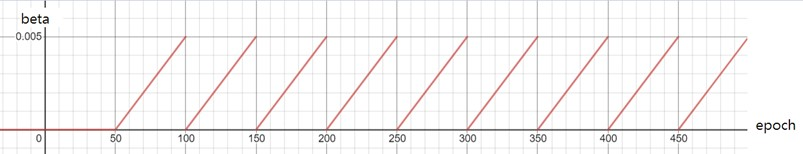
\includegraphics[width=\linewidth]{fig/10.jpg}
    \caption{訓練資料組,由左至右分別為模糊高度圖、衛星空照圖及真實高度圖}
    \label{fig:10}
\end{figure}

此外,訓練資料集共有3158組圖像,train資料集的資料對數為2526組,而test資料集為632組,總共為3158組圖像。

\subsection{訓練模型}
因本研究的模型結構是在pix2pix模型的基礎上修改,額外加上style encoder,所以pix2pix的部分仍然沿用論文作者的程式碼,進行訓練及測試時也是使用pix2pix原作者所提供的程式。

\noindent 訓練參數如下:
\begin{itemize}
\item Epoch:500
\item Batch size:18
\item Learning rate:0.0002 (前300 epoch),由0.0002線性下降至0 (後200 epoch)
\item Beta (為KLD的乘數,用來限制latent code分布的loss):隨時間的變化如圖十
\end{itemize}
	
\noindent 訓練時對資料組做的data augmentation (資料增強) 如下:
\begin{itemize}
\item 對模糊高度圖、衛星空照圖及真實高度圖同時作用的data augmentation:
	\begin{itemize}
		\item 50 \% 的機率上下翻轉
		\item 50 \% 的機率水平翻轉
		\item 50 \% 的機率轉置XY座標(斜向翻轉)
	\end{itemize}
	\item 對模糊高度圖及真實高度圖同時作用的data augmentation:
	\begin{itemize}
		\item 隨機縮放:將整張圖的像素值都乘以$e^x, x \sim N(0,0.0225)$ ($\mu$為0,$\sigma^2$為$0.0225$的高斯分布)
		\item 隨機偏值:將整張圖的像素值都增加$x, x\sim N(0,4)$
	\end{itemize}
\end{itemize}



\section{研究結果與討論}
\label{sec:res}
\subsection{評斷生成對抗網路模型的方法}
一般來說,很難找到一個好的方法來評斷生成對抗網路的表現,因為它不像一般的分類器能利用分類的精確度來評斷神經網路的優劣。

在本研究中,我們將會利用比較輸出與目標輸出的L1 Loss、L2 Loss、Perceptual Loss、FID、SSIM Index (structural similarity index)及生成每張圖像所需之平均時間來探討物理侵蝕模型、基礎的pix2pix模型與本研究模型的差異

\subsubsection{L1 Loss}
L1 Loss的計算方式是將兩張大小相同圖像所相對應的像素值相減後取絕對值,再相加在一起,最後取平均。具體公式如式~\ref{eq:2}~:
\begin{equation}
    \mathrm{L} 1 \operatorname{Loss}(X, Y)=\frac{1}{h \times w}\left(\sum_{i=1}^{h} \sum_{j=1}^{w}\left|X_{i, j}-Y_{i, j}\right|\right)
    \label{eq:2}
\end{equation}

其中,h, w分別為圖片的高度及寬度。可以發現L1 Loss的數值越小,代表兩張圖越相近。藉由L1 Loss我們可以看出兩張圖的相似程度。

\subsubsection{L2 Loss}
L2 Loss與L1 Loss的計算方式相似,只是將絕對值替換成平方,具體計算公式如式~\ref{eq:3}~:
\begin{equation}
    \mathrm{L} 2 \operatorname{Loss}(X, Y)=\frac{1}{h \times w}\left(\sum_{i=1}^{h} \sum_{j=1}^{w}\left(X_{i, j}-Y_{i, j}\right)^{2}\right)
    \label{eq:3}
\end{equation}

與L1 Loss相似,L2 Loss同樣是數值越小,代表兩張圖越相近,我們也可以透過L2 Loss來看出兩張圖的相似程度。但是L2 Loss對於偏離越多的值,會造成平方效果的改變。

\subsubsection{Perceptual Loss}

在計算Perceptual Loss\cite{zhang2018perceptual}時,會利用到一個已經訓練好(pre-trained)的VGG16模型。Perceptual Loss的計算方式是計算兩張圖像在VGG16各層activation的L1 Loss,最後再將各層計算出的L1 Loss相加。從Perceptual Loss可以看出兩張圖的風格是否相似,且Perceptual Loss同樣是數值越小,代表兩張圖越相近。

\subsubsection{FID (Fréchet Inception Distance)}
在計算FID (Fréchet Inception Distance)\cite{DOWSON1982450}時,會利用到一個已經訓練好 (pre-trained)的inception network v3神經網路來提取兩張圖片的特徵(feature)。圖片的特徵(為一個2048維的高階特徵)主要可以從inception network輸出層的前一層提取到。對於目標輸出,我們可以假設這個2048維向量是服從高斯分布。那由神經網路輸出的特徵應該也要服從高斯分布。所以我們知道生成對抗網路的目標是使這兩個分布的距離盡量接近。

而計算這兩個分布的距離等同於求目標輸出和輸出的2048維特徵的距離。數學上,如果想要計算兩個分布的距離,我們可以使用Fréchet distance來進行計算。

在計算上,我們會假設這兩個分布是服從高斯分布,且我們知道若一個隨機變數服從於高斯分布,則這個隨機變數可以使用高斯分布的標準差與平均表示,只要兩個分布的標準差和平均皆相同,則兩個分布相同。標準差和平均就是用來計算FID。但因為這裡我們要計算的是多維的向量,所以我們會使用平均和共變異數(covariance)矩陣來計算兩個分布的距離。而平均的維度是2048維,而共變異數矩陣就是一個$2048 \times 2048$維的矩陣。有了以上的定義後,我們就可以使用式~\ref{eq:4}~來計算輸出與目標輸出的FID。


\begin{equation}
    \mathrm{FID}(X, Y)=\left\|\mu_{X}-\mu_{Y}\right\|_{2}^{2}+\operatorname{Tr}\left(\Sigma_{X}+\Sigma_{Y}-2\left(\Sigma_{X} \Sigma_{Y}\right)^{\frac{1}{2}}\right)
    \label{eq:4}
\end{equation}

\subsubsection{SSIM index (structural similarity index)}
SSIM指標\cite{wang2004image}是一種用來評斷兩張圖像相似程度的方法,相較於其他種方法SSIM指標能更好的符合人眼對圖像品質的判斷。
SSIM指標主要透過比較兩張圖片的亮度、對比度及結構(structure)來評斷兩張圖片的相似程度,具體計算方式如式~\ref{eq:5}~:
\begin{equation}
    \begin{array}{l}
        \operatorname{SSIM}(X, Y)=[l(X, Y)]^{\alpha}[c(X, Y)]^{\beta}[s(X, Y)]^{\gamma}, \\
        l(X, Y)=\frac{2 \mu_{x} \mu_{y}+c_{1}}{\mu_{x}^{2}+\mu_{y}^{2}+c_{1}}, c(X, Y)=\frac{2 \sigma_{x} \sigma_{y}+C_{2}}{\sigma_{x}^{2}+\sigma_{y}^{2}+C_{2}}, s(X, Y)=\frac{\sigma_{x y}+C_{3}}{\sigma_{x} \sigma_{y}+c_{3}}
    \end{array}
    \label{eq:5}
\end{equation}
$l(X,Y)$是用來比較$X$, $Y$兩張圖的亮度,$c(X,Y)$則是用來比較對比度,而$s(X,Y)$用來比較兩張圖的結構。$\mu_x,\mu_y$代表兩張圖像素值的平均,$\sigma_x,\sigma_y$代表兩張圖像素值的標準差,$\sigma_{xy}$為兩張圖的共變異數(covariance),$C_1,C_2,C_3$是三個常數,以避免出現分母0的情況。另外,在本研究中,我們設定$\alpha=\beta=\gamma=1$。

根據以上的公式,我們可以發現SSIM index滿足對稱性($\operatorname{SSIM}(X,Y)=\operatorname{SSIM}(Y,X)$)、有界性($-1\leq \operatorname{SSIM}(X,Y)\leq 1$)及極限值唯一($\operatorname{SSIM}(X,Y)=1 \Longleftrightarrow X=Y$)

\subsubsection{生成每張圖像所需的平均時間}

我們利用PyTorch內建的\texttt{torch.cuda.Event()}來計算生成圖像所需的時間。計算完生成總時間後,就可以算出生成單張圖像所需的平均時間。在本研究中,我們是利用一張Nvidia GTX 1080 Ti 12 GB的顯示卡來進行圖像的生成。

\subsection{貼圖模型之訓練結果}

表二為原pix2pix結構與VAE-pix2pix結構的貼圖模型的測試結果,其圖像皆為來自test資料集之圖像,也就是說模型並沒有在訓練過程中“看過”這些圖像。藉由觀察這些圖像,我們可以更好的評斷模型的學習程度。表三則為兩個模型在test資料集的平均指標值。

\begin{table}[H]
    \centering
    \caption{原pix2pix及VAE-pix2pix的生成衛星空照圖的測試結果}
    \label{tab:2}
    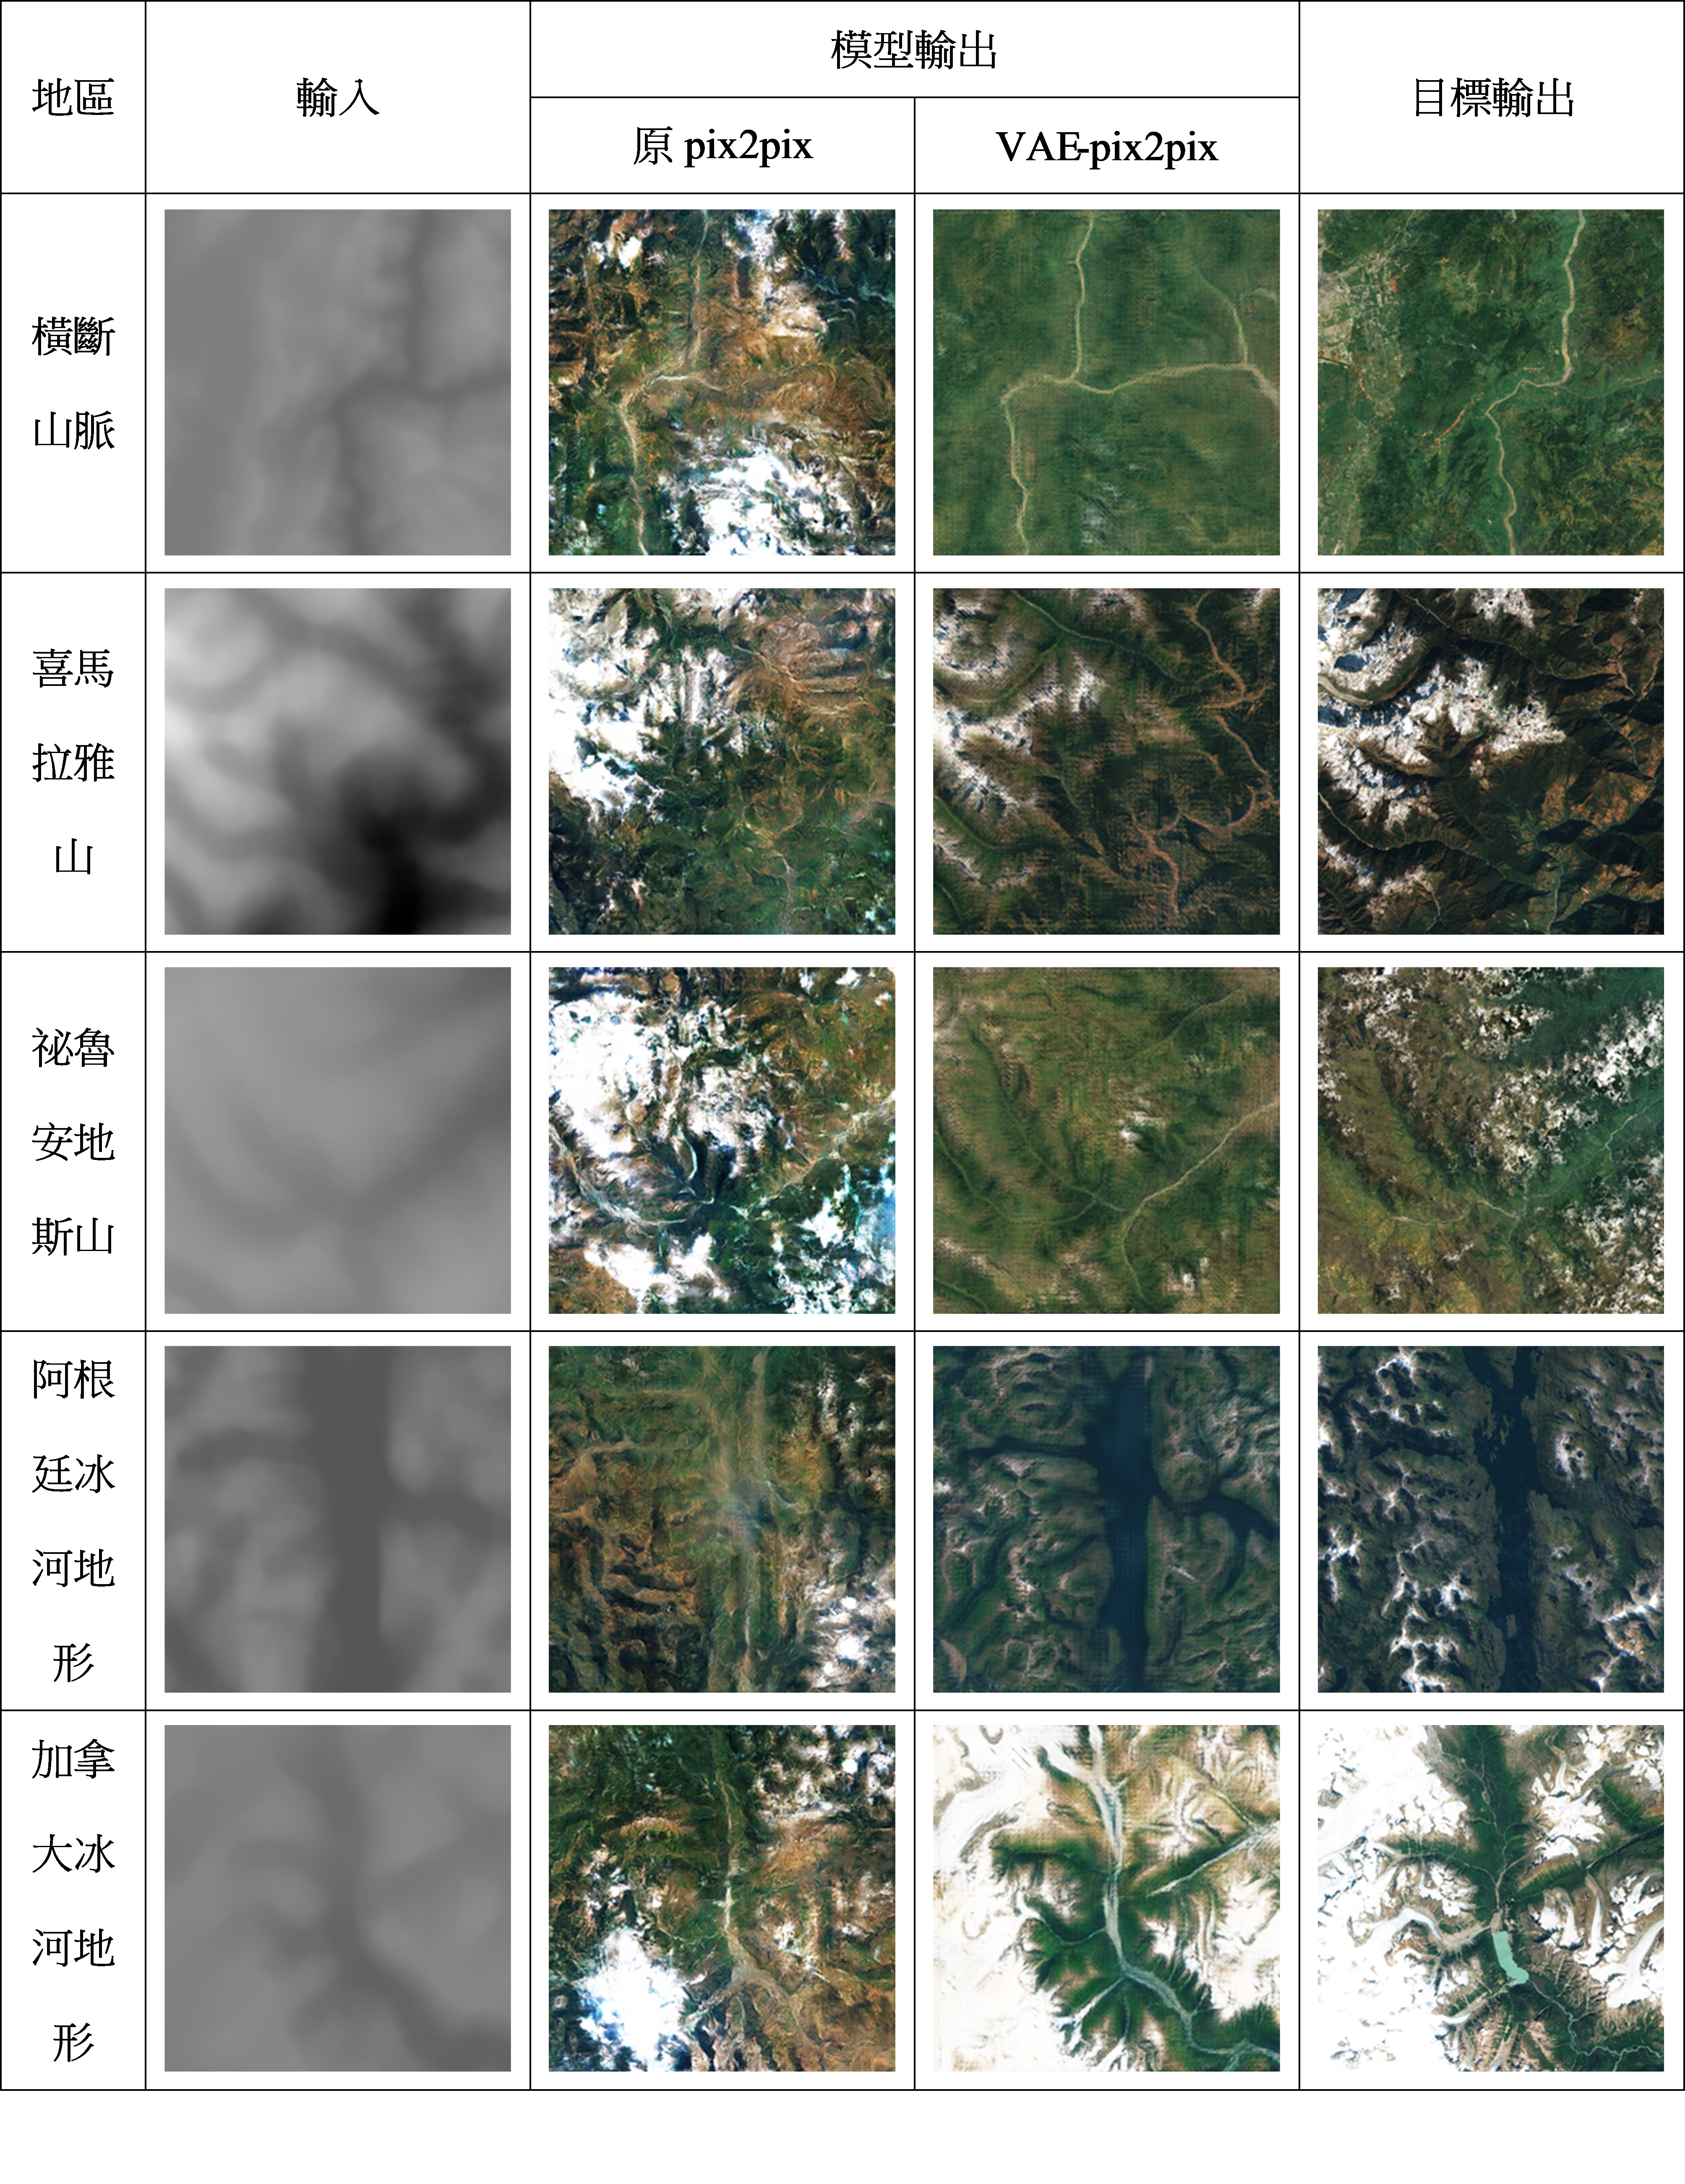
\includegraphics[width=0.8\linewidth]{fig/tab2.jpg}
\end{table}

\begin{table}[H]
    \caption{原pix2pix及VAE-pix2pix生成衛星空照圖的平均指標值}
    \label{tab:3}
    \begin{tabularx}{\linewidth}{|Y|Y|Y|Y|Y|Y|Y|}
        \hline
        \textbf{模型} & \textbf{L1 Loss} & \textbf{L2 Loss} & \textbf{Perceptual Loss} & \textbf{FID}    & \textbf{SSIM} & \textbf{平均生成時間(毫秒)} \\ \hhline{|=|=|=|=|=|=|=|}
        原pix2pix     & 61.176            & 6987.011         & 4.358 & \textbf{117.008} & 0.1076         & \textbf{13.925}              \\ \hline
        VAE-pix2pix   & \textbf{29.969}  & \textbf{2134.224} & \textbf{2.897}          & 121.742        & \textbf{0.2816} & 54.253                      \\ \hline
    \end{tabularx}
\end{table}


可以發現我們建構的VAE-pix2pix架構相較於原pix2pix架構生成出的衛星空照圖較接近於目標輸出,不僅山脈的顏色更接近於目標輸出,且輸出的空照圖相當符合輸入高度圖的結構。這點也反映在各指標上,L1 Loss、L2 Loss、Perceptual Loss及SSIM都表現較好。

\subsection{地形擬真模型之訓練結果}

測試圖像都是來自test資料集。測試完成後,測試結果如表四,我們會將模型輸出與目標輸出計算出各指標,如表五,藉此來判斷每個模型的表現。

\begin{table}[H]
    \centering
    \caption{物理侵蝕模型、原pix2pix結構及VAE-pix2pix結構的生成地形高度圖的測試結果}
    \label{tab:4}
    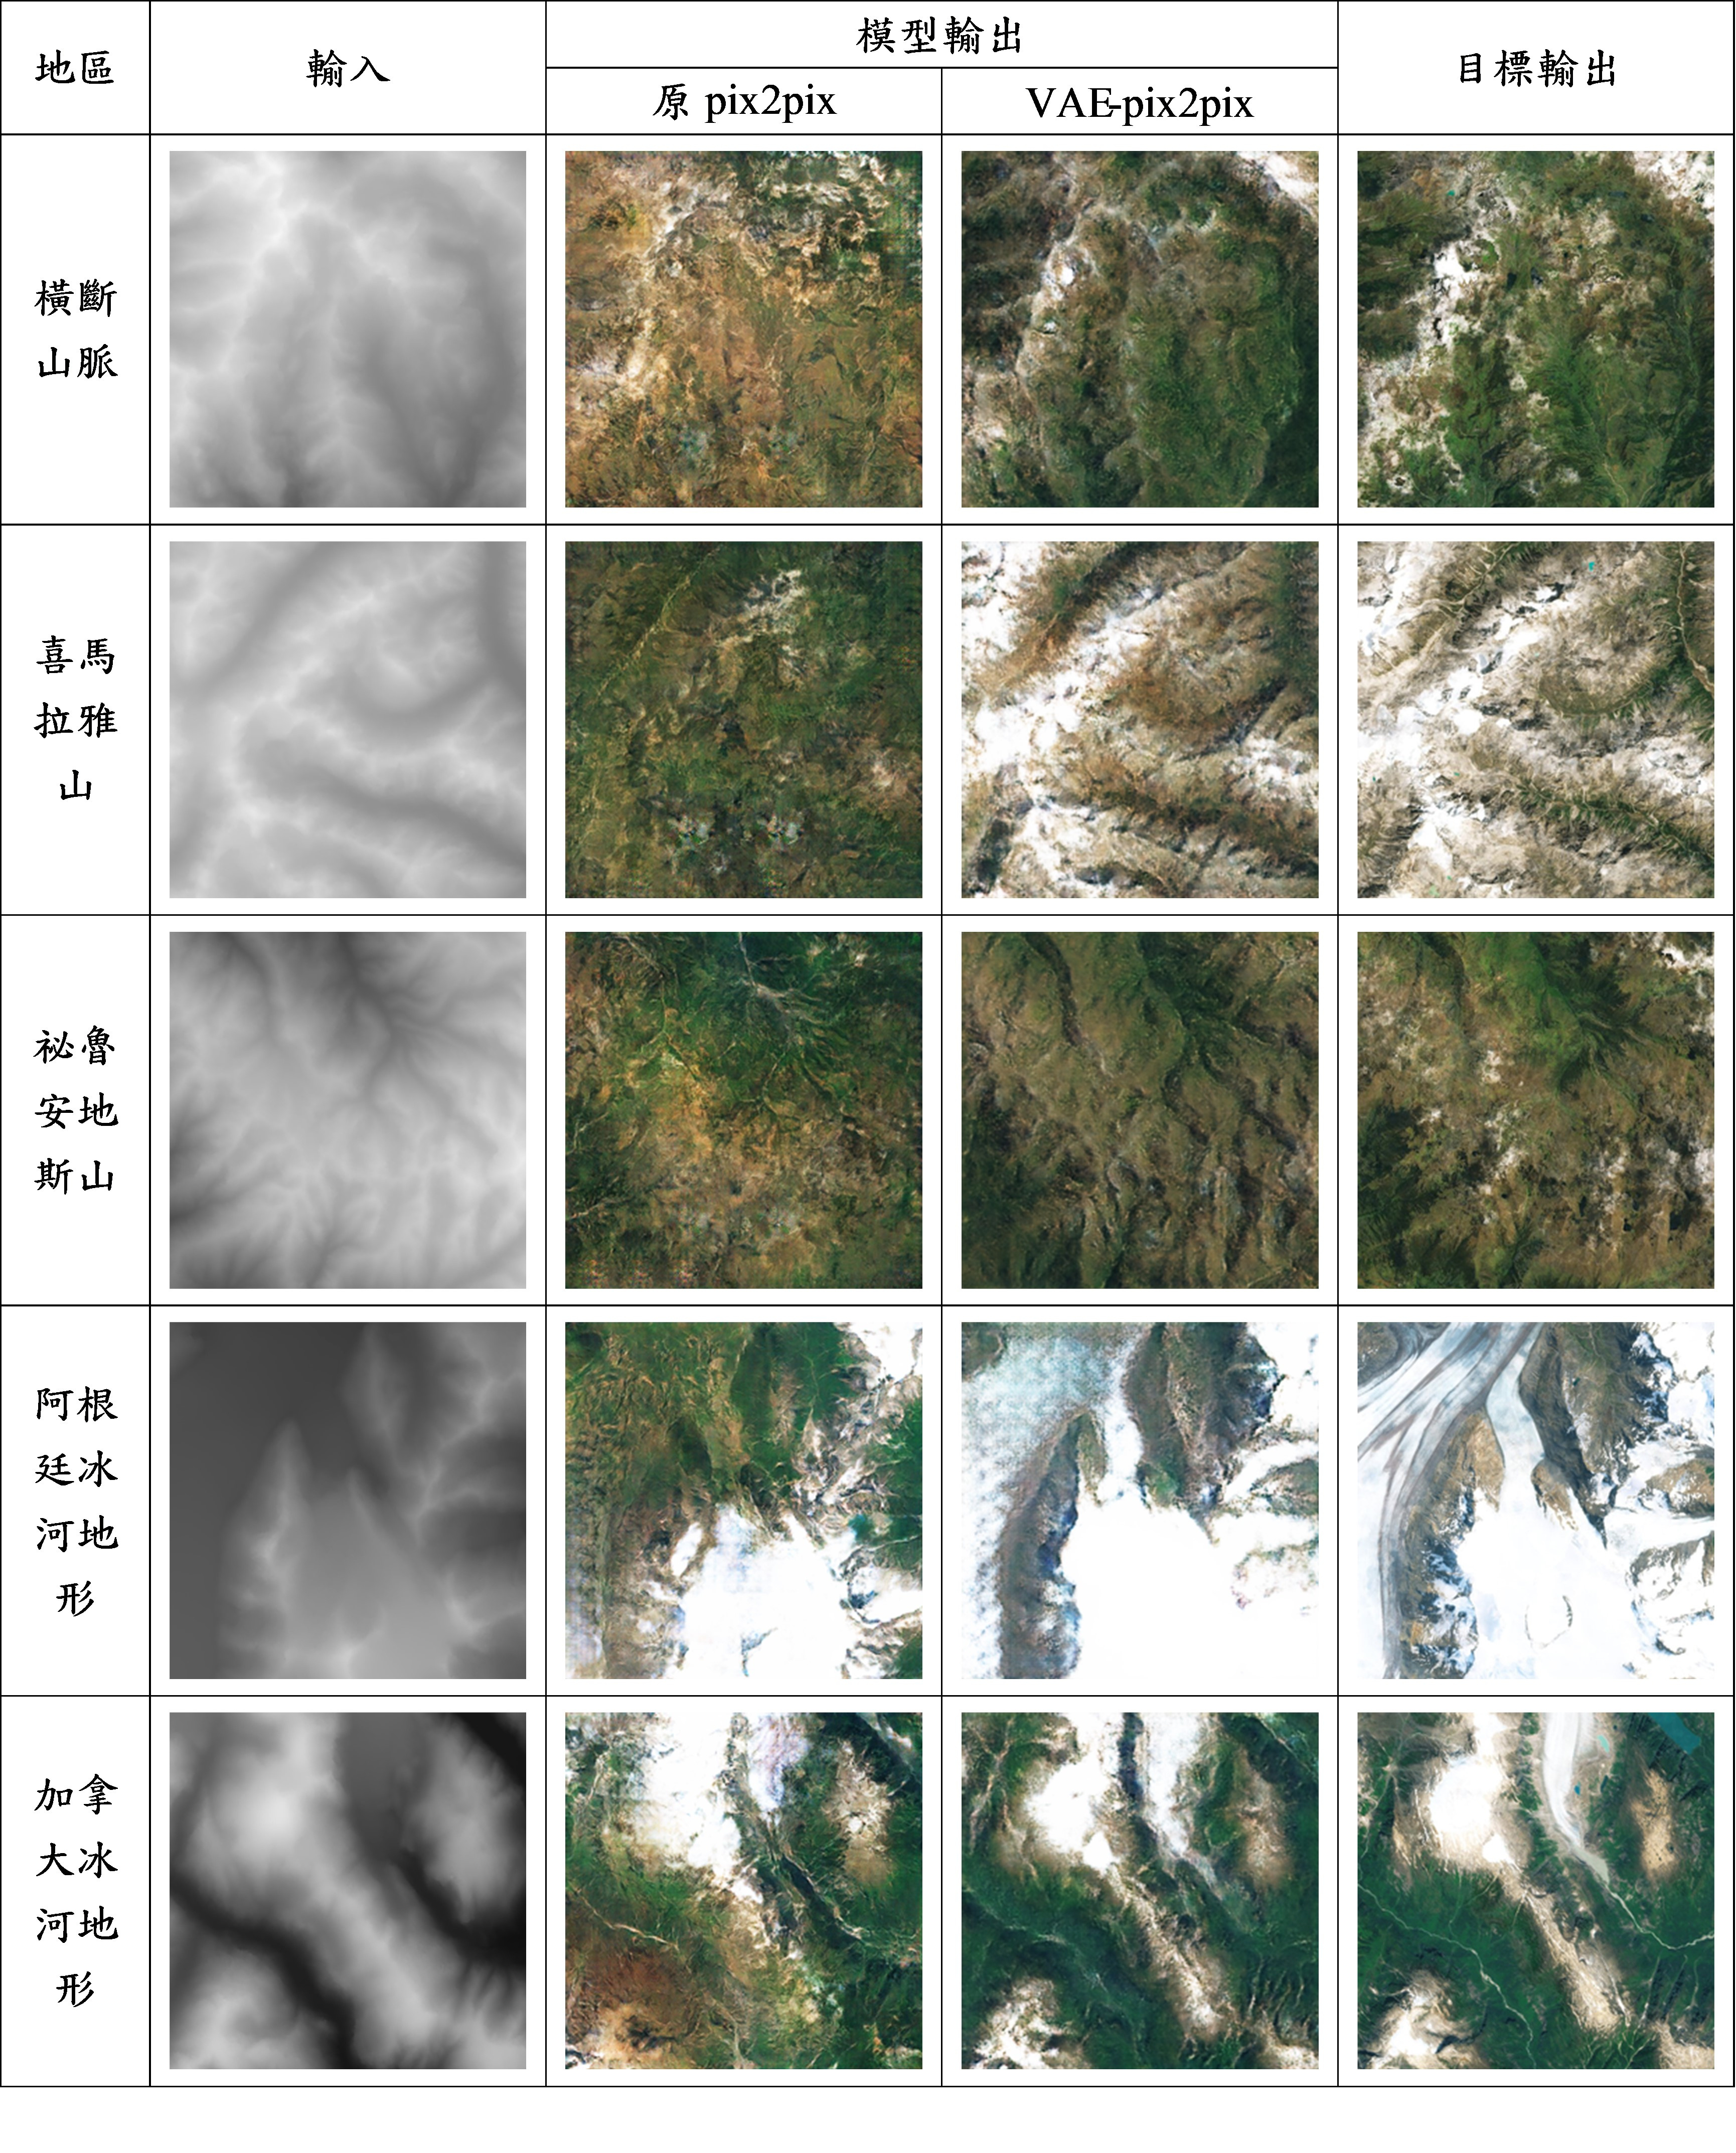
\includegraphics[width=0.9\linewidth]{fig/tab4.jpg}
\end{table}

\begin{table}[H]
    \caption{物理侵蝕模型、原pix2pix及VAE-pix2pix在test資料集的平均指標值}
    \label{tab:7}
    \begin{tabularx}{\linewidth}{|Y|Y|Y|Y|Y|Y|Y|}
        \hline
        \textbf{模型} & \textbf{L1 Loss} & \textbf{L2 Loss} & \textbf{Perceptual Loss} & \textbf{FID}    & \textbf{SSIM}  & \textbf{平均生成時間(毫秒)} \\ \hhline{|=|=|=|=|=|=|=|}
        物理侵蝕模型  & 14.335            & 335.69          & 1.3168 & 138.260 & 0.7499         & 340.199                       \\ \hline
        原pix2pix     & 7.09            & 107.478         & 1.5114 & 184.077 & 0.7411         & \textbf{13.925}              \\ \hline
        VAE-pix2pix   & \textbf{4.311}   & \textbf{48.567}   & \textbf{1.1382}           & \textbf{89.971} & \textbf{0.882} & 54.253                     \\ \hline
    \end{tabularx}
\end{table}

從表五,我們可以發現VAE-pix2pix生成的高度圖較原pix2pix所生成的圖像來說更接近於目標輸出。由各指標也可以看到VAE-pix2pix要優於pix2pix。相較於物理侵蝕模型,本研究的方法約比其生成的速度快6倍。

\subsection{各地區的高度圖及空照圖在latent space上的分布}
latent code的分布是判斷VAE訓練結果好壞的重要觀察項目。在本研究中尋找最佳模型參數的階段,使latent code的分布合理是我們的主要目標之一,因為「不好的」latent code分布代表模型沒有正常處理風格資訊。

我們從五個地區蒐集的每個資料組(由模糊高度圖、衛星空照圖及真實高度圖組成),經過訓練好的VAE-pix2pix中style encoder的轉換,會被一一映射到8維的latent space上,如下圖。每個點代表一個資料組,而點的顏色代表所在地區。而因為latent code其實是一個高斯分布,圖中資料點顯示的位置只取高斯分布的中心位置。

我們從以下兩點觀察latent code分布的好壞:
\begin{enumerate}
\item 不同地區的latent code是否分離:

由圖十一可以看出,每個地區的latent code都大致自成一個色塊,表示style encoder\textbf{能很好的分辨每種地區地形的不同特徵}。

\item 所有latent code是否集中:

由圖十一可以看出,大部分的資料點都集中成同一個連續區塊,表示在應用時,沿一個連續的路徑調整輸入的latent code,生成出的地形\textbf{風格能連續的轉換},且藉由插值兩種地區的latent code,我們的模型可以生成出\textbf{「兩種風格的中間」}的地形,這點也反映在圖十七的測試上。不過一部分的阿根廷和加拿大冰河地形的latetnt code跑到遠處,這個問題可能要再調整beta等參數來解決。
\end{enumerate}

\begin{figure*}
    \centering
    \begin{subfigure}[b]{0.475\textwidth}
        \centering
        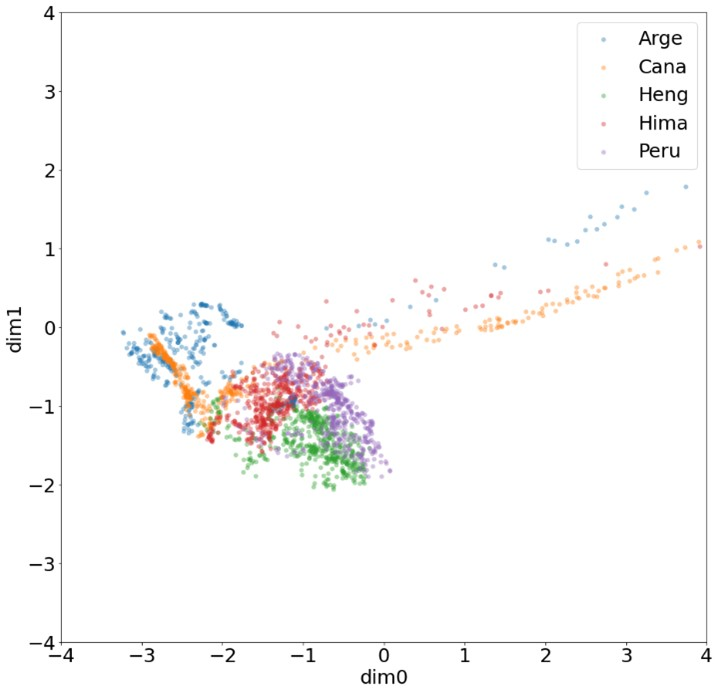
\includegraphics[width=\textwidth]{fig/12a.jpg}
        \caption[]%
        {{\small}}
        \label{fig:14}
    \end{subfigure}
    \hfill
    \begin{subfigure}[b]{0.475\textwidth}
        \centering
        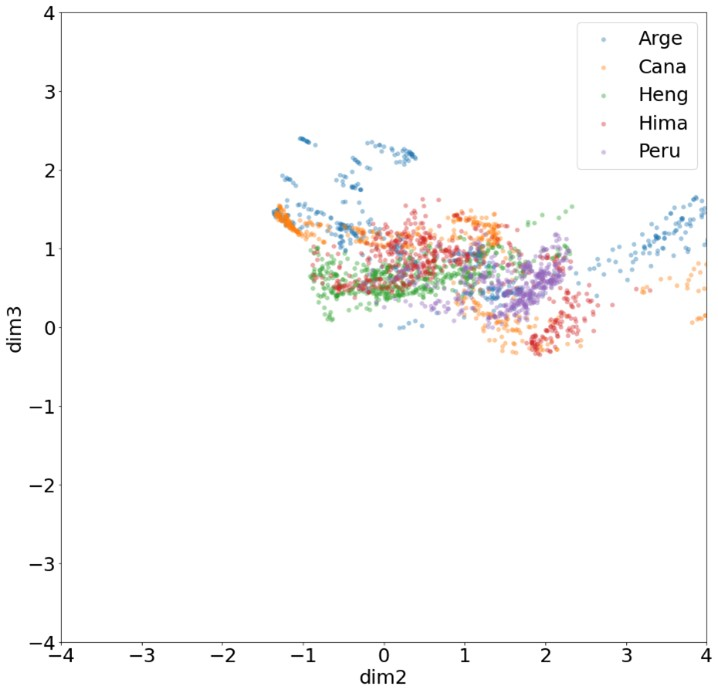
\includegraphics[width=\textwidth]{fig/12b.jpg}
        \caption[]%
        {{\small}}
        \label{fig:15}
    \end{subfigure}
    \vskip\baselineskip
    \begin{subfigure}[b]{0.475\textwidth}
        \centering
        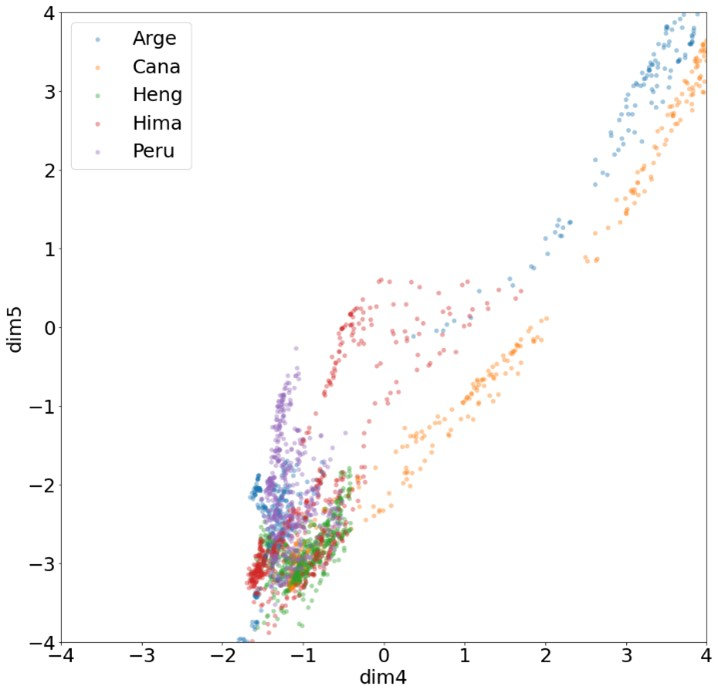
\includegraphics[width=\textwidth]{fig/12c.jpg}
        \caption[]%
        {{\small}}
        \label{fig:16}
    \end{subfigure}
    \hfill
    \begin{subfigure}[b]{0.475\textwidth}
        \centering
        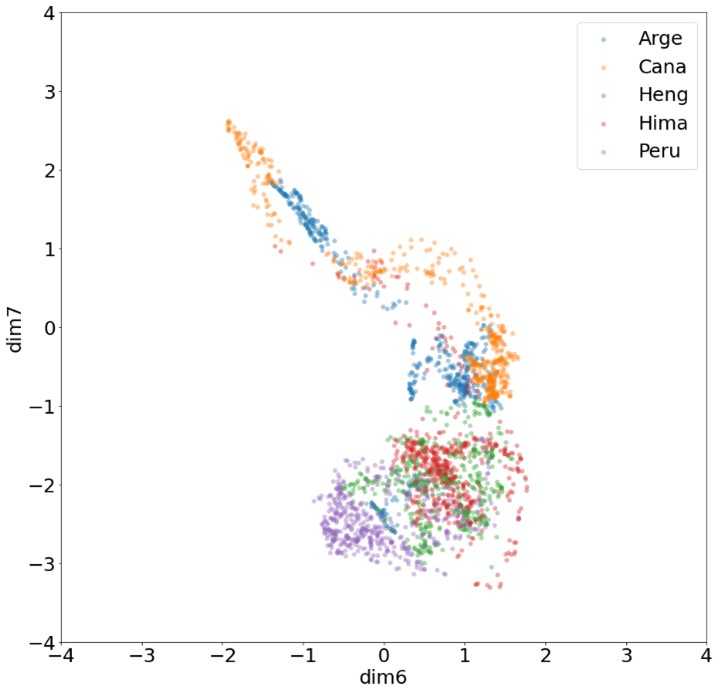
\includegraphics[width=\textwidth]{fig/12d.jpg}
        \caption[]%
        {{\small}}
        \label{fig:17}
    \end{subfigure}
    \caption[ The average and standard deviation of critical parameters ]
    {\small 將資料組透過 style encoder 轉換後映射到 8 維 latent space 上}
    \label{fig:latent}
\end{figure*}


\subsection{建構模型的API伺服器}
為了避免每次需要應用各模型處理高度圖時都要重新載入模型,我們利用Python的Flask套件建立了一個API伺服器,並將其建置於工作站上。用戶可以直接上傳手繪的高度圖,並在伺服器上用訓練好的各模型進行處理,後再回傳回用戶端。不僅運算快速,且也省去了架設軟體環境和下載模型檔案的時間。這個API可以快速的在模型之間切換,且支援本研究中所有訓練的模型。

\subsection{Unity用戶端}

本研究自行開發了一個Unity客戶端,使用戶可以在Unity Editor的編輯模式中直接對地形進行操作。使用者可以匯入一張高度圖或直接在地形上繪製3D的模型。每當畫完一筆畫後,Unity會直接對API伺服器送出請求,並在一秒內更新出擬真的山脈地形。也可以將貼圖模型所生成的擬真衛星空照圖貼在3D模型上,具體功能如圖十二、圖十三、圖十四、圖十五:



\begin{figure*}
    \centering
    \begin{subfigure}[b]{0.475\textwidth}
        \centering
        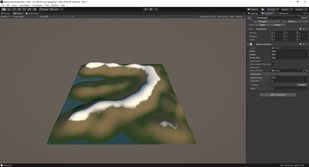
\includegraphics[width=\textwidth]{fig/13.jpg}
        \caption[]%
        {{\small Unity客戶端的初始畫面}}
        \label{fig:13}
    \end{subfigure}
    \hfill
    \begin{subfigure}[b]{0.475\textwidth}
        \centering
        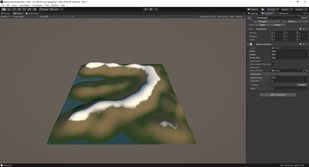
\includegraphics[width=\textwidth]{fig/14.jpg}
        \caption[]%
        {{\small 用戶手繪之大致地形}}
        \label{fig:14}
    \end{subfigure}
    \vskip\baselineskip
    \begin{subfigure}[b]{0.475\textwidth}
        \centering
        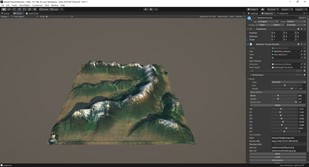
\includegraphics[width=\textwidth]{fig/15.jpg}
        \caption[]%
        {{\small VAE-pix2pix生成的擬真地形}}
        \label{fig:15}
    \end{subfigure}
    \hfill
    \begin{subfigure}[b]{0.475\textwidth}
        \centering
        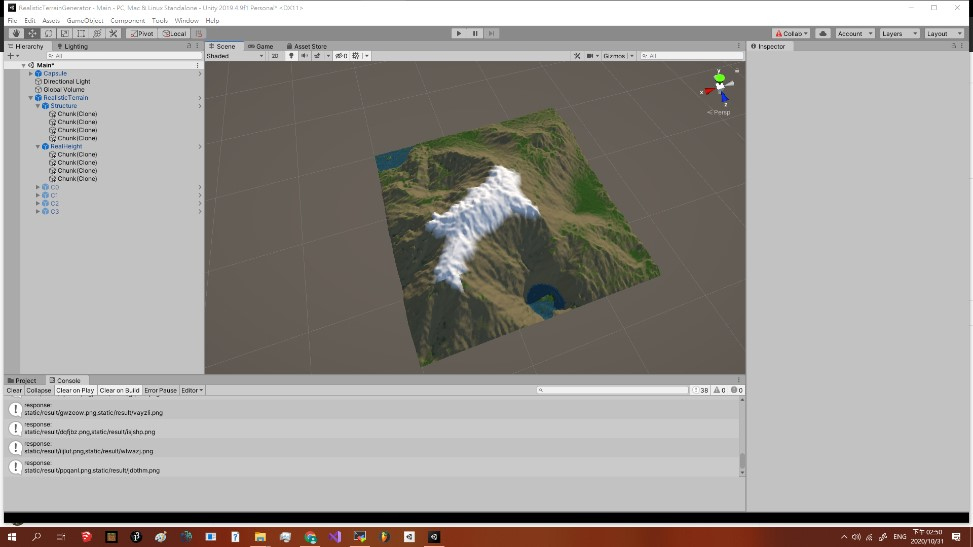
\includegraphics[width=\textwidth]{fig/16.jpg}
        \caption[]%
        {{\small 將生成的空照圖貼在擬真地形}}
        \label{fig:16}
    \end{subfigure}
    \caption[ The average and standard deviation of critical parameters ]
    {\small Unity客戶端功能}
    \label{fig:unity}
\end{figure*}

\subsection{由用戶端調整latent code對於輸出風格的效果}
圖十六展示了以256 x 256的橫斷山脈模糊高度圖為輸入高度圖,並在圖上不同區域使用不同的地區的風格,分別為阿根廷、加拿大、喜馬拉雅和秘魯。圖十六的中央為四個地區在latent space上的平均,而往左下為加拿大、右下為阿根廷、右上為喜馬拉雅、左上為秘魯的風格。可以發現四個方向的生成風格都有不同,且與真實地區的空照圖相似。

\begin{figure}[H]
    \centering
    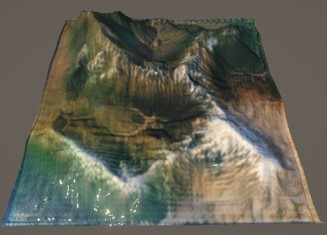
\includegraphics[width=0.7\linewidth]{fig/17.jpg}
    \caption{在空間上展示不同風格的輸出}
    \label{fig:17}
\end{figure}

精確來說,圖十七中的latent code設置為:
定左下角座標為$(0,0)$,右上角座標為$(1,1)$,加拿大、祕魯、阿根廷、喜馬拉雅的地區的平均latent code分別為 $a,b,c,d$ ,則$(x,y)$處latent code $= 3((1-x)(1-y)a + (1-x)yb + x(1-y)c + xyd)-\frac{2(a+b+c+d)}{4}$。所以在接近中心處的latent code為四個地區latent code之間的內插值;在靠近邊緣及角落處的latent code則為平均latent code往四個地區latent code 的外推(extrapolation)。圖十八顯示了本研究的模型將pix2pix與style encoder結合後,使生成的地形不侷限於訓練資料的風格,能生成出其他未出現在訓練資料集,甚至不真實存在的地形風格,這項特性大大增加了模型的應用價值。

在應用上,使用者也可以利用VAE-pix2pix這項能在空間上設定不同latent code的特性,增加設計地形的自由度。


\subsection{透過改變style encoder的輸入改變輸出圖像的風格}
為了測試以上的討論,我們將一張高度圖及多張與此張高度圖不互相對應的空照圖一起輸入到VAE-pix2pix的style encoder中,驗證能改變輸出圖像的風格。表六為測試的結果:

\begin{table}[H]
    \centering
    \caption{將同一張高度圖與不同的空照圖作為style encoder的輸入,並比較其輸出}
    \label{tab:6}
    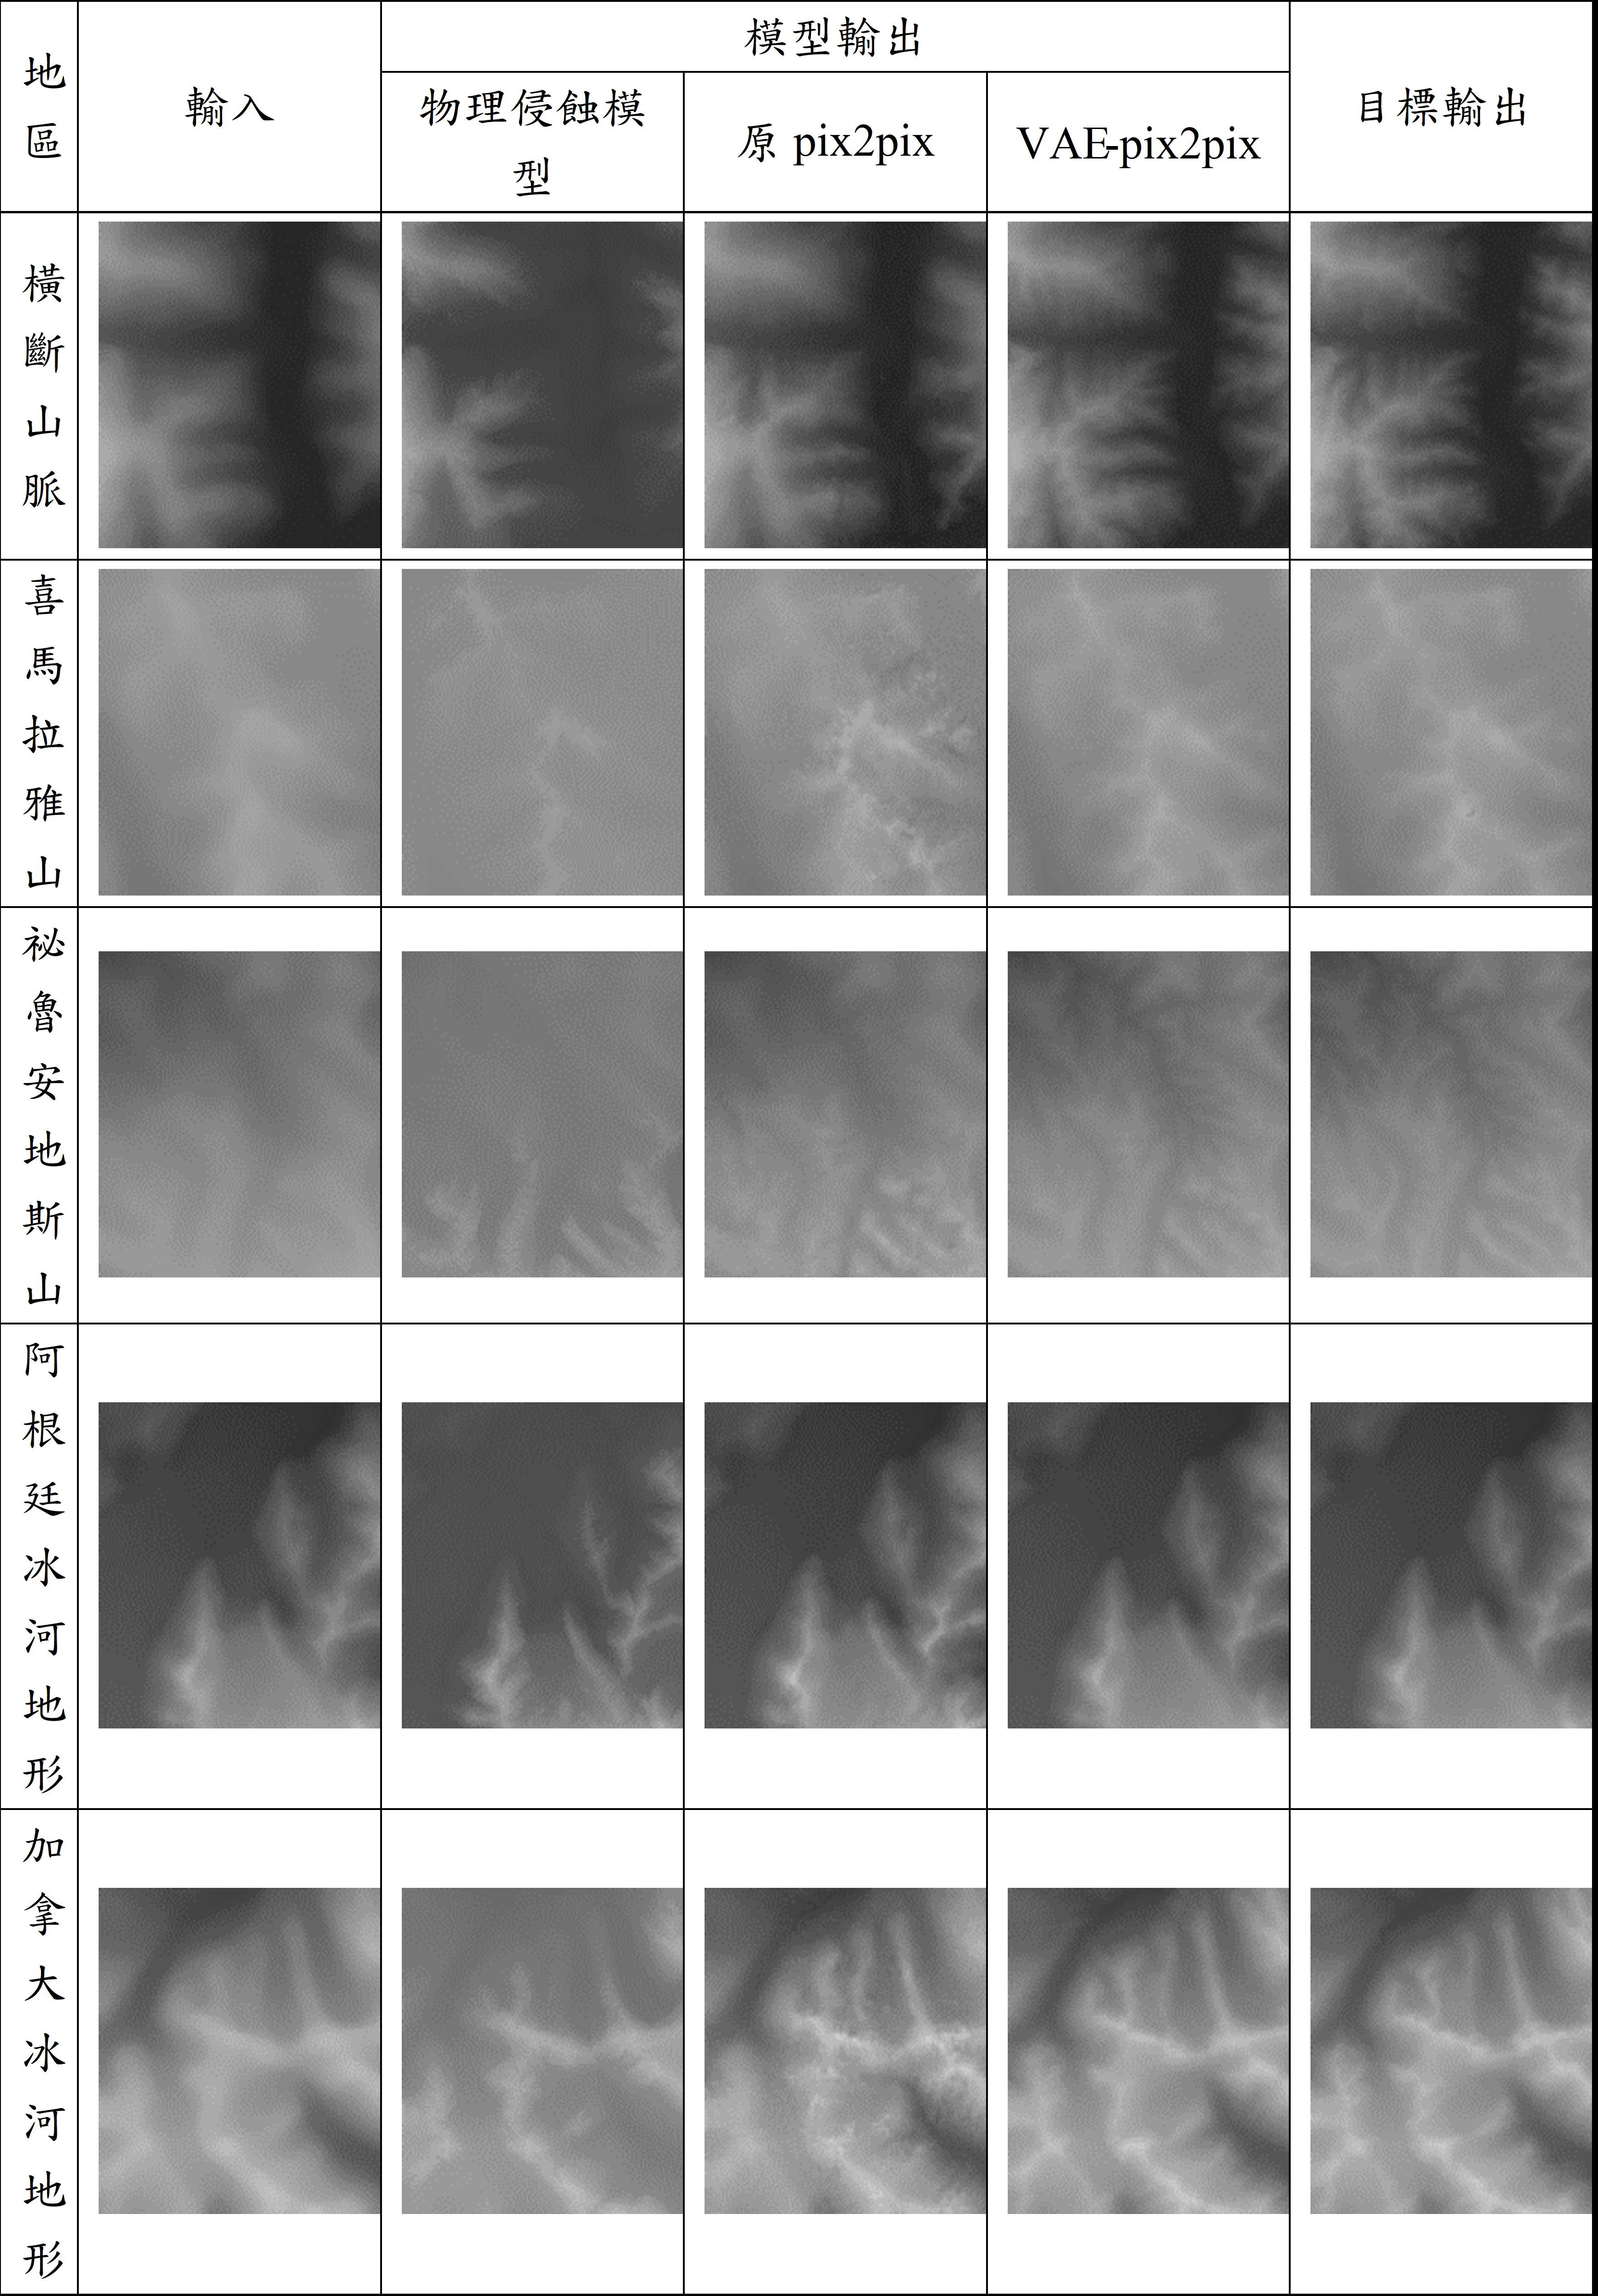
\includegraphics[width=0.8\linewidth]{fig/tab6.jpg}
\end{table}

可以發現VAE-pix2pix模型可以很好的將輸入空照圖的特徵提取出來,且也可以保留高度圖上河流及山脊等特徵。

\subsection{討論物理侵蝕模型、pix2pix模型及VAE-pix2pix之間的差異}
表~\ref{tab:9}~比較了物理侵蝕模型、原pix2pix模型及本研究建構的VAE-pix2pix模型之間的差異。

雖然VAE-pix2pix模型的生成速度慢於原pix2pix模型,但其所生成圖像的品質為三者最優,還可以透過改變latent code的數值,改變生成山脈地形的風格。
\begin{table}[H]
    \caption{物理侵蝕模型、原pix2pix模型及VAE-pix2pix的比較}
    \label{tab:9}
    \begin{tabularx}{\linewidth}{|Y|Y|Y|Y|Y|}
        \hline
        \textbf{模型}   & \textbf{功能}                                              & \textbf{生成速度} & \textbf{生成品質} & \textbf{是否可以改變生成圖像的風格} \\ \hhline{|=|=|=|=|=|}
        物理侵蝕模型    & 將大致高度圖經過侵蝕後變得較為擬真                         & 慢(約300毫秒)       & 最差              & 否                                  \\ \hline
        原pix2pix模型   & 將大致高度圖變得更為擬真、根據高度圖生成相對應的衛星空照圖 & 最快(約7毫秒)     & 其次              & 否                                  \\ \hline
        VAE-pix2pix模型 & 將大致高度圖變得更為擬真、根據高度圖生成相對應的衛星空照圖、改變生成圖像的風格 & 快 (約10毫秒)     & 最好              & 是                                  \\ \hline
    \end{tabularx}
\end{table}
\section{結論與應用}

在本研究,我們利用NASA的SRTM 1 Arc-Second及MapTiler收集了全球五個地區的高度圖及相對應的空照圖。利用這些收集的圖像,訓練了自行建構的VAE-pix2pix模型。VAE-pix2pix為Variational Autoencoder (VAE)及pix2pix結合的模型,可以將人工繪製的高度圖自動加上真實山脈應有的細節(包含尖銳的山脊、山壁上的紋路、連續的河流網路等……),也能生成相對應的擬真衛星空照圖。

經過實測,相較於原pix2pix模型,VAE-pix2pix所生成的高度圖及空照圖會更接近於真實世界的山脈高度圖,且VAE-pix2pix模型也可以透過改變其latent code的數值來生成出不同風格的高度圖及衛星空照圖,如地貌的顏色或雪線的高度等,這些都能增加模型生成圖像的多樣性,甚至能以可能不真實存在的風格生成地形,讓應用更為廣泛。與物理侵蝕模型進行比較,不僅生成速度遠快於物理侵蝕模型,生成品質也更為擬真,這些都是優於傳統模型的地方。

為了使模型的使用更加簡單,不用在終端機上打入許多複雜的指令,我們將模型的使用包裝成Unity客戶端,Unity客戶端可以在圖形使用者介面完成在模糊高度圖加上山脈細節的工作,並能直接在畫面上顯示3D模型,也可以將生成出的衛星空照圖貼在擬真地形的3D模型中,使空照圖及高度圖能更好的呈現。

綜合以上,本研究的VAE-pix2pix模型可以生成出更為擬真的高度圖及空照圖,且還能自由調整生成圖像的風格。而我們開發的Unity客戶端,可以使我們的模型直接應用於遊戲的開發中,也使得原先需要分成兩個步驟的生成擬真的山脈地形與生成相對應的空照圖整合為一個步驟。這些都會讓遊戲開發生成擬真山脈模型的任務變得十分容易。


\nocite{*}
\printbibliography[title={參考文獻}]

\addcontentsline{toc}{section}{參考文獻}


\newpage
\begin{appendices}
    \setcounter{page}{1}
    \textbf{\LARGE 附錄}

    \section{高度圖及空照圖的具體收集範圍}
    如內文所提,我們會利用高度圖左下角的經緯度座標表示一張高度/空照圖,如一張高度圖是由25°N, 98°E、25°N, 99°E、24°N, 99°E、24°N, 98°E四個座標點所圍成的範圍,則此張高度圖的檔名即為N24E98。除了會在下面列出各個座標點,我們也有將具體的收集範圍在地圖上框出。

    \subsection{中國橫斷山脈}
    \begin{multicols}{4}
        \begin{enumerate}
            \item N27E099
            \item N27E098
            \item N26E101
            \item N26E100
            \item N26E099
            \item N26E098
            \item N29E101
            \item N29E100
            \item N29E099
            \item N29E098
            \item N28E101
            \item N28E100
            \item N28E099
            \item N28E098
            \item N27E101
            \item N27E100
        \end{enumerate}
    \end{multicols}
    \begin{figure}[H]
        \centering
        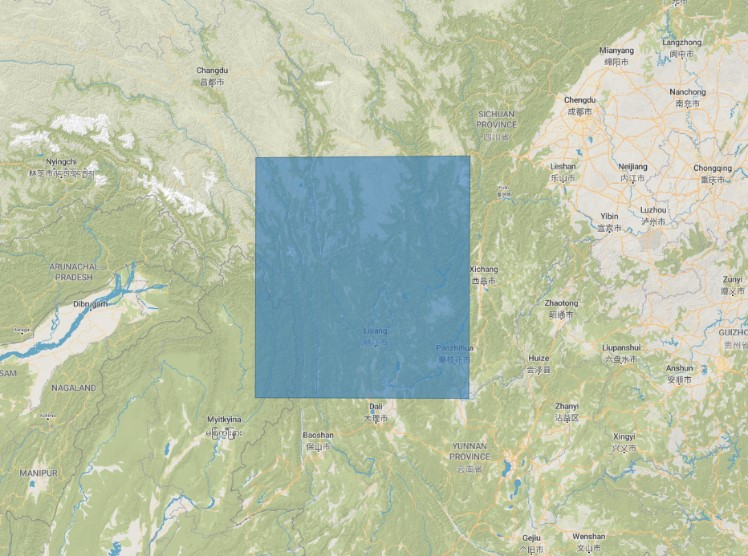
\includegraphics[width=0.8\linewidth]{fig/a1.jpg}
    \end{figure}
    \subsection{喜馬拉雅山脈}
    \begin{multicols}{4}
        \begin{enumerate}
            \item N29E081
            \item N29E082
            \item N29E083
            \item N28E083
            \item N28E084
            \item N28E085
            \item N27E085
            \item N27E086
            \item N28E086
            \item N27E087
        \end{enumerate}
    \end{multicols}
    \begin{figure}[H]
        \centering
        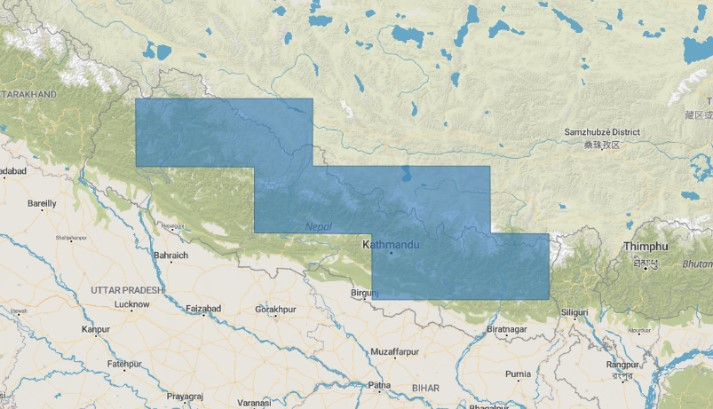
\includegraphics[width=0.8\linewidth]{fig/a2.jpg}
    \end{figure}
    \subsection{祕魯安地斯山脈}
    \begin{multicols}{4}
        \begin{enumerate}
            \item S07W079
            \item S08W079
            \item S08W078
            \item S09W078
            \item S10W078
            \item S10W077
            \item S11W077
            \item S12W077
            \item S12W076
            \item S13W076
            \item S14W076
            \item S14W075
            \item S15W075
            \item S15W074
            \item S16W073
        \end{enumerate}
    \end{multicols}
    \begin{figure}[H]
        \centering
        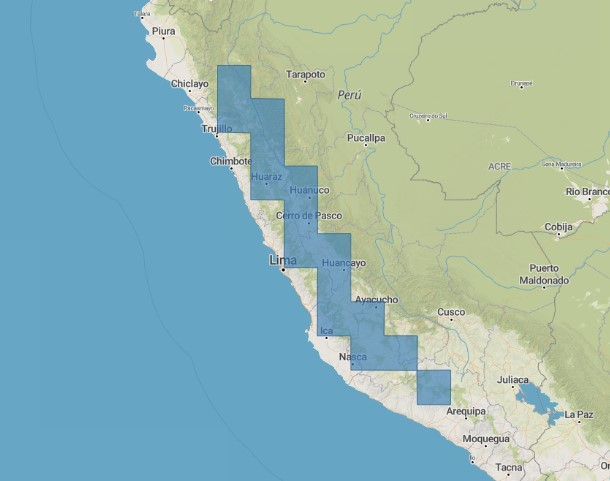
\includegraphics[width=0.8\linewidth]{fig/a3.jpg}
    \end{figure}
    \subsection{阿根廷冰河}
    \begin{multicols}{3}
        \begin{enumerate}
            \item S48W074
            \item S49W074
            \item S49W075
            \item S50W074
            \item S50W075
            \item S51W073
            \item S51W074
            \item S51W075
            \item S52W074
        \end{enumerate}
    \end{multicols}
    \begin{figure}[H]
        \centering
        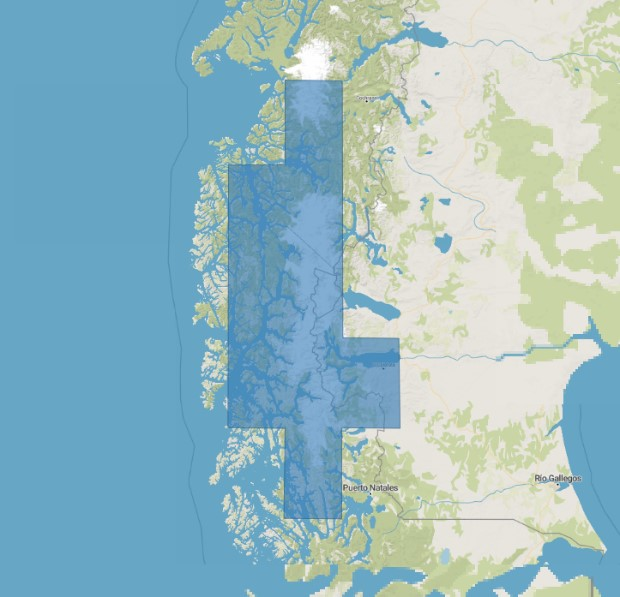
\includegraphics[width=0.8\linewidth]{fig/a4.jpg}
    \end{figure}
    \subsection{加拿大冰河}
    \begin{multicols}{3}
        \begin{enumerate}
            \item N58W134
            \item N57W133
            \item N56W132
            \item N56W131
            \item N55W131
        \end{enumerate}
    \end{multicols}
    \begin{figure}[H]
        \centering
        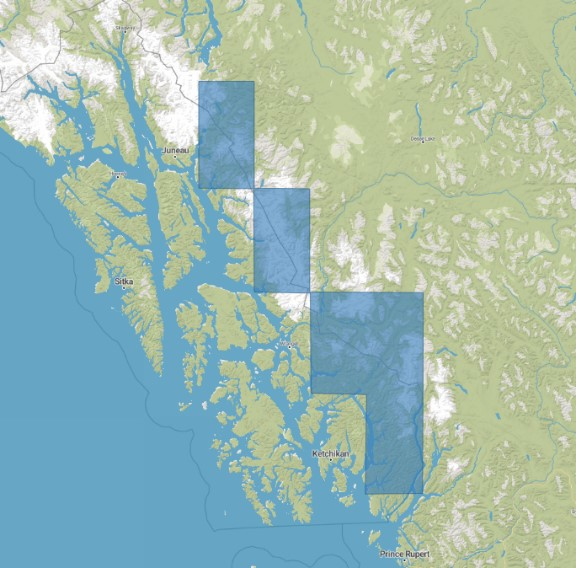
\includegraphics[width=0.8\linewidth]{fig/a5.jpg}
    \end{figure}
\end{appendices}

\end{document}